\section{Algorithm construction}
\label{cha:Algorithm_construction}
In this section algorithm construction will be presented. In this thesis four
algorithms were used for pattern recognition task. Here we start with the basic
algorithm of rough sets, later present rough sets algorithm with modification
step and at last multistage hybrid algorithm consisting of genetic algorithm,
rough sets and fuzzy logic will be shown in greater details. 
\subsection{Rough sets algorithm construction}
\label{cha:Algorithm_construction_rough_set}
The basic rough sets algorithm with constant step of granulation
can be summarized in six steps:
\begin{enumerate}
    \item If the attributes are the real numbers then the granulation preprocessing 
        is needed first. After this step, the value of each attribute is represented 
        by the number of interval in which this attribute is included. For each
        attribute from $l=(1, \ldots , q)$ we choose the same numbers of
        intervals $K_l$ called step of granulation $G$. For the $l$-th attribute 
        denoted by $v^l_{p_l}$ define
        its $p_l$ interval from $p_l=(1, \ldots, K_l)$
    \item Using training dataset construct set $FOR(C)$ of decision rules of
        the following form:
        $$IF \, (x^1 = v_{p_1}^1) \, AND \, (x^2=v_{p_2}^2) \, AND \, \ldots \,
        (x^q=v_{p_q}^q) \, THEN \, \Psi(S, x)=j$$
        Each generated rule is evaluated and strength factor is assigned
        accuracy of approximation (see section \label{cha:Rough_sets_indicators})
    \item For the created set of formulas $FOR(C)$ for each $j=1, \ldots, m$ we
        calculate lower, upper approximation and the boundary region.
    \item In order to classify pattern $x$ we look for matching rules in the
        set $FOR(C)$ (the left condition is fulfilled by its attributes).
    \item If there is only one matching rule, then we classify this pattern $x$ 
        to the class  which is indicated by its decision attribute $j$, 
        because for sure such rule is belonging to the lower approximation of all rules 
        indicating $j$, this rule is certain.
    \item If there is more then one matching rule in the set $For(C)$, 
        it means that the recognized pattern should be classified by the 
        rules from the boundary regions and in this case as a decision we 
        take the index of boundary region for which the strength of corresponding 
        rule is maximal. In such a case we take into account the rules which are possible.
    \item In other cases: no rule was found or few rules have the same strength
        factor unknown pattern $x$ is rejected.
\end{enumerate}
\subsection{Rough sets algorithm construction with modification of decision rules}
\label{cha:Algorithm_construction_rough_set_modification}
It can happen that for certain number of intervals we cannot find patterns in
the learning set so as a consequence we generate dummy rule, useless in the
classification process. The main drawback of algorithm presented in \label{cha:Algorithm_construction_rough_set}
that is starts with an arbitrary step of granulation and its accuracy strongly
depends on it. In this section the recursive modification of the previous algorithm is
presented allowing for automatically changing the step of granulation is
pattern $x$ is rejected. The modification is as follows:
\begin{enumerate}
    \item Algorithm starts with an arbitrary chosen step of granulation.
        Generally, it is a high value to ensure that recursion can be invoked
        by decreasing $G$ value. Shortly speaking, we divide every domain of feature into $G$
        intervals. The whole procedure 1-6 is repeated from the previous point.
    \item If for the pattern $x$ we cannot find neither certain nor possible
        decision rule, it means that algorithm cannot find proper representation 
        in learning set. Then we try to find matching rule by increasing recursively
        the current interval for every condition attribute $l=1, \ldots, q$ and
        the learning procedure is invoked once again until the proper rule is
        found.  
    \item Recursive algorithm stops if for every attribute $G=1$. Then the
        decision is taken randomly.
    \item To enhance the process of finding proper decision formula for
        different $G$ the decision set $FOR(C)$ for the certain $G$ are stored
        in the memory.
\end{enumerate}

\subsection{Fuzzy logic algorithm construction}
\label{cha:Algorithm_construction_fuzzy_logic}
\subsubsection{Problem formulation}
\label{cha:Fuzzy_logic_basic_problem_formulation}
In the fuzzy logic algorithm one of the most important key is creation of rule
which will ensure proper classification. When we have no expert knowledge about
dataset it is not an easy task to generate them on its own. In the literature
one can find many practical examples of how to generate $IF-THEN$ rules, from
the statistical tools to heuristic algorithms. In this thesis genetic
algorithm will be used to generate rule set as one of the approach in the
recent year (more information about genetic algorithm can be found in section
\ref{cha:Genetic_algorithm}).
For the algorithm construction we have to make few assumptions:
\begin{itemize}
    \item The same as for rough sets algorithm, we assume that we have $N$
        training patterns.
    \item A set $F$ of linguistic values and their membership functions is given
        for describing each attribute. 
\end{itemize}
I think that the second point requires in-depth explanation. First of all how
to partition each attribute into linguistic values and how to describe each
membership function. Here is the place for genetic algorithm to find optimal
parameters. 
\begin{figure}[H]
    \begin{center}
        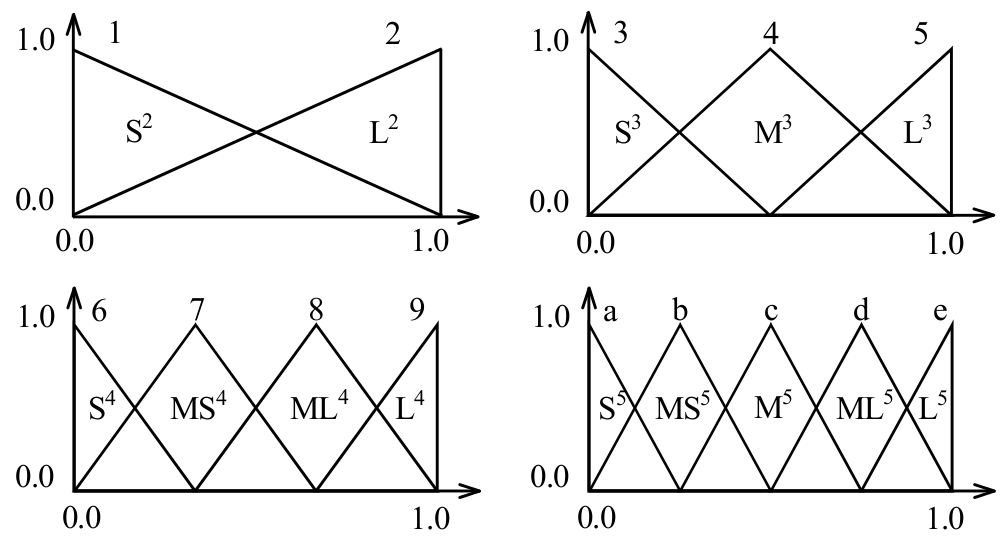
\includegraphics[width=\textwidth]{fig/fuzzy_example.png}
    \end{center}
    \caption{Example fuzzy partition set for an attribute}
    \label{fig:fuzzy_example}
\end{figure}
Fig. \ref{fig:fuzzy_example} shows an example how to generate fuzzy set $F$ of
possible membership functions. In this example $14$ membership functions can be
used. Each function has a subscript defining its linguistic value. To emphasize
with which problem we facing with let take into account that each attribute is divided 
in the same way as depicted in Fig. \ref{fig:fuzzy_example}. Having
$d$-dimensional feature space possible combination of membership functions for
rule generation is equal to $14^d$. To evaluate each solution is
computationally impossible in a reasonable time. 

In this section we reconsider fuzzy rules in the following form:
$$IF\, x_1=A_{q1}\, AND\, x_2=A_{q2}\, AND\, \ldots\, AND\, x_d=A_{qd}\, THEN\,
class\, C_q\, with \, CF_q$$
where $x=(x_1, x_2, \ldots, x_d)$ is a $d$-dimensional pattern vector; $A_{qi}$
is an antecedent fuzzy set with a linguistic label (taking into account the
example from \ref{fig:fuzzy_example} $A_{qi}$ can be one label from the set
$\{1, 2, \ldots, 9, a, b, \ldots, e \}$); $C_q$ is a consequent class and can
have value one of $\{1, \ldots, m\}$, $CF_q$ is a rule strength determined in the
training phase (see more in section \ref{cha:Fuzzy_logic_rule_generation}); $q$
determines the number of rule from the set $\{1, \ldots, N_{rule}\}$, generally
$N_{rule}$ is about ten or twenty. Rule strength $CF_q$ is used in the
defuzzyfication process.
\subsubsection{Rule generation}
\label{cha:Fuzzy_logic_rule_generation}
The process of rule generation for fuzzy logic without the expert knowledge is
complex and done in couple steps. To construct fuzzy rule we use available
training set. Let say that at first we generate randomly $N_rule$ rules. For
each training pattern $x_p$ calculate the compatibility grade of a single rule
connected with antecedent part $A_q = (A_{q1}, A_{q2}, \ldots, A_{qd})$ using
the product operator of each membership function $\mu_{A_{qi}}$ determined for
$A_{qi}$:
\begin{equation}
    \mu_{A_q}(x_p)=\mu_{A_q1}(x_p)\cdot\mu_{A_q2}(x_p)\cdot\ldots\mu_{A_qd}(x_p)
    \label{eq:mu_product}
\end{equation}
If we know how to calculate the compatibility grade of each training pattern
now we can determine $C_q$ and $CF_q$ for each rule. The fuzzy probability
$P(class\, h|A_q)$ of class $h$, $h=(1, \ldots, m)$ is given by eq. (\ref{eq:fuzzy_probability})
\begin{equation}
    Pr(class \, h|A_q) = \frac{\sum\limits_{x_p \in class\,
    h}\mu_{A_q}(x_p)}{\sum\limits_{p=1}^m\mu_{A_q}(x_p)}
    \label{eq:fuzzy_probability}
\end{equation}
For the rule $R_q$ the label of class is assigned according to eq.
(\ref{eq:fuzzy_max})
\begin{equation}
    R_q: C_q = max\limits_{h=\{1, \ldots, m\}}\{Pr(class\,h|A_q)\}
    \label{eq:fuzzy_max}
\end{equation}
In the learning phase it can happen that that rule $R_q$ can be activated by
patterns coming from different classes. We have to determine the strength
factor for this rule if we have chosen a proper class $h$ for rule $R_q$. 
\begin{equation}
    R_q: CF_q=Pr(class\, h|A_q) - \sum\limits_{h=1, h\neq C_q}^MPr(class\,h|A_q)
    \label{eq:fuzzy_strength}
\end{equation}
If $CF_q$ in eq. (\ref{eq:fuzzy_strength}) is negative then rule $R_q$ is
denoted as dummy and not used in later reasoning.
\subsubsection{Fuzzy reasoning}
\label{cha:Fuzzy_reasoning}
Let assume that $N_{rule}$ fuzzy rules are generated with indicators $C_q$,
$CF_q$ determined by eq. (\ref{eq:fuzzy_max}, \ref{eq:fuzzy_strength}). Then
the process of classification is done as follows:
\begin{equation}
    \Psi(S, x_p) =  C_q \leftarrow max_{h=\{1,\ldots, M\}}\{\mu_{A_{q}}(x_p)\cdot CF_q\}
    \label{eq:fuzzy_classification}
\end{equation}
The label of the class for unknown pattern is determined by a winner rule $R_w$
that has the maximum compatibility grade and the rule strength $CF_q$.

If multiple fuzzy rules have the same maximum product $\mu_{A_q}$ but different
consequent classes then the classification is rejected. The same action is
taken if no fuzzy rule is compatible with the incoming pattern $x_p$. 
\subsubsection{Genetic algorithm for  fuzzy algorithm construction}
\label{cha:Fuzzy_logic_genetic_algorithm}
In this section genetic algorithm will be described in greater details. This
algorithm was used to generate initial number $N_{rule}$ of fuzzy rules for
classification. 
Basic assumptions:
\begin{itemize}
    \item Fuzzy rule encoding is the same as presented in section \ref{cha:Fuzzy_logic_basic_problem_formulation}
    \item Training data set is given
    \item Triangular membership functions are used and described by 2-tuple
        $(a, b)$, where $a$ is the center value, and
        $b$ determines left and right extend of function respectively.
        \begin{equation}
            f(x) = 
            \begin{cases}
                \frac{-1}{b}\cdot x + \frac{a+b}{b} &
                x \geq a \, and \, x \leq (a+b) \\
                \frac{1}{b}\cdot x - \frac{a-b}{b} &
                x \geq (a - b)\, and\, x < a \\
                0 & otherwise
            \end{cases}
            \label{eq:fuzzy_function}
        \end{equation}
    \item Possible partitions of the feature space are determined in the same
        way as in the example presented in fig. \ref{fig:fuzzy_example}
    \item Genetic algorithm uses standard operations such as cross\_over,
        mutation, population generation, fitness evaluation.
    \item As the template for genetic fuzzy algorithm Mitchigan approach was
        used which means that we have $N_{rule}$ number of individuals in the
        population
\end{itemize}
Next few step will present the whole structure of genetic algorithm used in
this section:
\begin{itemize}
    \item Chromosome representation and encoding: 
        \begin{itemize}
            \item Each individual represents a single fuzzy rule $R_q$.
                The length of the chromosome is the same as the number of 
                attributes describing the pattern $x$. Each allele has value
                determining which linguistic variable is used in the current
                rule. Reconsider Iris dataset which is a $4$-dimensional
                classification problem and that for each attribute $14$
                membership functions plus one variable telling to omit the
                attribute (called $DON'T \,USE$). An exemplary individual can be as follows:
                $$1|c|DON'T \;USE|4||1|0.85$$
                Above individual can be decoded into rule presented in fig.
                \ref{fig:fuzzy_rule}
                \begin{figure}[H]
                    \begin{center}
                        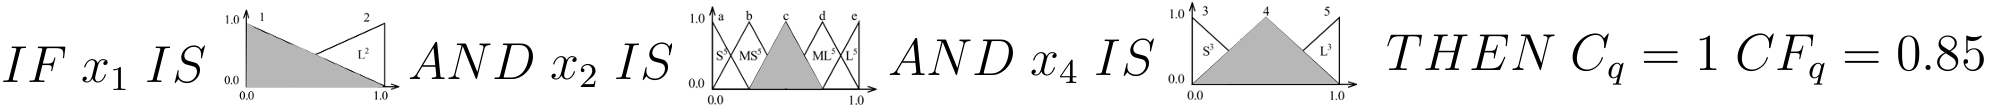
\includegraphics[width=\textwidth]{fig/fuzzy_rule.png}
                    \end{center}
                    \caption{Example rule decoded from the individual
                    chromosome (attribute $x_3$ was omitted in this rule)}
                    \label{fig:fuzzy_rule}
                \end{figure}  
        \end{itemize}
    \item Individual evaluation
        \begin{itemize}
            \item To ensure proper genetic algorithm process an appropriate
                fitness function must be defined. Firstly the nature of pattern
                recognition task must be taken into account and secondly the
                structure of the fuzzy algorithm. Generally, we aiming at
                generating rule with the highest $CF_q$ grade, smallest number
                of attributes and the highest classification rate. Fitness
                function is given by eq. (\ref{eq:fuzzy_fitness})
                \begin{equation}
                    F_{fg} = w_1\cdot NC + w_2\cdot NNC + (\frac{1}{NOF})^2 +
                    w_3\cdot CF
                    \label{eq:fuzzy_fitness}
                \end{equation}
                where $w_1$, $w_2$ are weights for a reward and punishment to
                the rule based on the classification result; $NC$, $NNC$ are
                the numbers of correctly recognized and misclassified patterns
                by a particular rule, respectively; $NOF$ is the number of
                attributes used by the rule (in the above example $NOF=3$);
                $CF$ is the strength factor of the rule and $w_3$ is the weight.
                The best individuals are those which maximize function $F_{fg}$
        \end{itemize}
    \item Cross-over, mutation and population generation
        \begin{itemize}
            \item From the whole population two individuals were chosen
                randomly to constitute father and mother parent. With a
                probability of $0.5$ each allele was picked either from mother
                or father chromosome. In this way we generate two new
                individuals.
            \item In the particular generation one chromosome is chosen
                randomly and later in each allele new membership function is
                taken from other possible function. For example is in the first
                allele the first membership function is chosen the set of
                candidates is given by $\{2, \ldots, 9, a, \ldots, e, DON'T\, USE\}$
            \item In genetic algorithm one of the most important issue is how
                to generate next population. Here, after the end of one
                generation individuals from the population are merged with
                those created through cross-over and mutation operations.
                Later, the average fitness value $F_{avg}$ is calculated in the whole
                set. To the next generation those individuals are passed which
                their fitness indicator $F$ is greater than the average $F \ge F_{avg}$
        \end{itemize}
\end{itemize}
Of course it can happen that for cross-over and mutation operator
newly-generated individual will be invalid (the whole chromosome contains only
$DON'T\; USE$ linguistic variables). In such a situation rule is rejected and
the whole generation process is repeated again.

Table \ref{tab:fuzzy_genetic_parameters} presents basic genetic algorithm parameters.
Optimal values were determined during simulations by trial and error method.
\begin{table}[H]
    \caption{Parameter settings for genetic algorithm used in fuzzy logic}
    \centering
    \begin{tabular}{|c|c|}
        \hline
        Parameter & value \\ \hline \hline
        $N_{rule}$ & 10 \\ \hline
        $N_{replace}$ & $N_{rule}/2$ \\ \hline
        Crossover probability & 0.9 \\ \hline
        Mutation probability & 0.3 \\ \hline
        Generations & 500 \\ \hline
    \end{tabular}
    \label{tab:fuzzy_genetic_parameters}
\end{table}
\subsection{Multistage hybrid algorithm construction}
\label{cha:Multistage}
In this section the main algorithm in this thesis will be described. 
\subsubsection{Motivations}
\label{cha:Mutlistage_motivations}
When we deal with complex data it can happen that a single classifier is not
sufficient. There arises a question if connection of different classifier will
improve the classification. In this thesis hybridization of rough sets and
fuzzy logic is presented. The next subsections show algorithm construction.
\subsubsection{Rough sets and genetic algorithm}
\label{cha:Multistage_rough_genetic}
Rough sets algorithm presented in section
\ref{cha:Algorithm_construction_rough_set} uses an arbitrary chosen step of
granulation which affects the accuracy of classification. Additionally, each
attribute uses the same granulation interval which in some cases gives good
results in other efficiency is low. Another drawback of the basic rough set
algorithm is that it uses all attributes for rule construction. 

Finding the optimal attribute reduct and rough set partition is $NP$ problem.
To overcome this obstacle a genetic algorithm was used in the similar way as in section
\ref{cha:Fuzzy_logic_genetic_algorithm}. Now, a single individual describes the
partition for each attribute independently. Reconsider individual encoding for
$4$-dimensional Iris dataset. The number of granulation for the attribute is
chosen from the set $\{1, 2, \ldots, K_{max}\}$, where $K_{max}$ is the maximum
value of discretization. Additionally, $DON'T\; USE$ variable is used to
determine that a given attribute is not used in the rule. The example of
individual is given below:
$$|2|DON'T \; USE|K_{max}|3||120$$
It means that the first feature is divided into two intervals, the second is
not used and the third and fourth are discretized into $K_{max}$ and 3
intervals respectively. The fitness indicator of this individual is $120$.
To evaluate individual the following fitness function given by eq.
(\ref{eq:rough_fitness}) is used.

\begin{equation}
    F_{rg} = w_1\cdot NC + w_2\cdot NNC + (\frac{1}{NOF}) +w_3\cdot (\frac{1}{NOCR})^2
    \label{eq:rough_fitness}
\end{equation}

where $w_1$, $w_2$ are weights for a reward and punishment to
the individual on the classification result; $NC$, $NNC$ are
the numbers of correctly recognized and misclassified patterns; $NOF$ is the number of
attributes used by the rule (in the example above $NOF=3$);
$NOCR$ is the number of certain rule which are derived from
partition given by the individual; $w_3$ is the weight.

The whole procedure can be summarized in few steps:
\begin{enumerate}
    \item Determine maximum partition value for each attribute $K_{max}$. In
        this thesis $K_{max}$ is the same for all features
    \item Generate $N_{pop}$ individuals by randomly assigning value from the
        set $\{1, 2, \ldots, K_{max}, \, DON'T\; USE\}$ to each allele
    \item Treat each individual as a rough set partition and calculate lower,
        upper approximation and boundary region. Evaluate individual using
        fitness function $F_{rg}$
    \item Generate $N_{replace}$ individuals using genetic operators and merge
        with the current population
    \item Choose $N_{pop}$ individual for the next generation
    \item If stopping criteria is not fulfilled go to $2$
\end{enumerate}
Parameters for genetic algorithm used in this section are presented in table
\ref{tab:rough_genetic_parameters}:
\begin{table}[H]
    \caption{Parameter settings for genetic algorithm used in rough sets}
    \centering
    \begin{tabular}{|c|c|}
        \hline
        Parameter & value \\ \hline \hline
        $N_{pop}$ & 10 \\ \hline
        $N_{replace}$ & $N_{pop}/2$ \\ \hline
        Crossover probability & 0.9 \\ \hline
        Mutation probability & 0.2 \\ \hline
        Generations & 100 \\ \hline
    \end{tabular}
    \label{tab:rough_genetic_parameters}
\end{table}
In case of genetic algorithm for rough set $100$ generations were sufficient to
obtain reliable results.
\subsection{Hybrid rough sets and fuzzy logic}
\label{cha:Multistage_rough_fuzzy}
Multistage classifier created in this thesis can be divided into three phases:
\begin{enumerate}
    \item Rough sets classifier construction using genetic algorithm presented
        in section \ref{cha:Algorithm_construction_rough_set}
    \item Fuzzy logic classifier construction with rule generation by heuristic
        approach described in \ref{cha:Fuzzy_logic_genetic_algorithm}
    \item Pattern recognition using hybrid classifier 
\end{enumerate}
Each step plays an important role in the whole process and affect the final
classification accuracy. Proper parameters of genetic algorithm are especially
important. The whole hybrid algorithm can be summarized in the following steps:
\begin{enumerate}
    \item Divide available dataset into three separated subsets: the first for
        genetic algorithm operation, the second and third as training and
        testing.
    \item Train rough sets, fuzzy logic classifiers
    \item Classify pattern using rough sets algorithm:
        \begin{itemize}
            \item If pattern is classified by a certain or possible rule then
                it is a final label
            \item If no rule were found or more than one rule have the same
                strength, but different label then pattern is rejected and
                processed by fuzzy logic classifier.
        \end{itemize}
\end{enumerate}
Illustrative scheme of hybrid classifier is presented in fig.
\ref{fig:schematic}
\begin{figure}[H]
    \begin{center}
        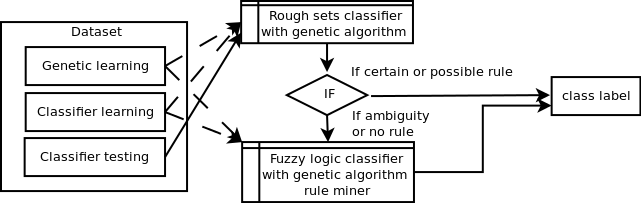
\includegraphics[width=\textwidth]{fig/diagram.png}
    \end{center}
    \caption{Schematic diagram how hybrid classifier works}
    \label{fig:schematic}
\end{figure}
